\documentclass[tikz,border=10pt]{standalone}
\usepackage{amsmath,amssymb}
\usepackage{tikz}
\usetikzlibrary{arrows,automata,backgrounds,calendar,chains,decorations,decorations.pathreplacing,decorations.text,fit,matrix,mindmap,patterns,petri,plotmarks,positioning,shadows,shapes,shapes.callouts,shapes.geometric,shapes.misc,spy,trees,calc,intersections,tikzmark,arrows.meta}
\usepackage{xcolor}
\usepackage{pgfplots}
\pgfplotsset{compat=1.16}

% Common math macros from the book
\def\x{\mathbf{x}}
\def\y{\mathbf{y}}
\def\z{\mathbf{z}}
\def\A{\mathbf{A}}
\def\b{\mathbf{b}}
\def\c{\mathbf{c}}
\def\w{\mathbf{w}}
\def\v{\mathbf{v}}
\def\u{\mathbf{u}}
\def\e{\mathbf{e}}
\def\zero{\mathbf{0}}
\def\R{\mathbb{R}}
\def\N{\mathbb{N}}
\def\Z{\mathbb{Z}}
\def\Q{\mathbb{Q}}
\def\st{\text{s.t.}}
\def\vect#1{\mathbf{#1}}
\def\xLP{x^{\mathrm{LP}}}
\def\zLP{z^{\mathrm{LP}}}
\def\xIP{x^{\mathrm{IP}}}

% Common node styles from the book
\tikzset{
    main/.style={circle, draw, fill=gray!20, minimum size=1cm, font=\normalsize},
    dot/.style={circle,fill=blue,minimum size=3pt,inner sep=0pt, outer sep=-1pt},
    vertex/.style={circle,fill=black!25,minimum size=20pt,inner sep=0pt},
    edge/.style={draw,-,thick},
    directed edge/.style={draw,->,>=latex,thick},
}

% Additional macros for 3D/coordinate systems
\newcommand{\xhat}{\hat{\x}}
\newcommand{\yhat}{\hat{\y}}
\newcommand{\zhat}{\hat{\z}}
\newcommand{\ihat}{\hat{\imath}}
\newcommand{\jhat}{\hat{\jmath}}
\newcommand{\khat}{\hat{k}}

\begin{document}
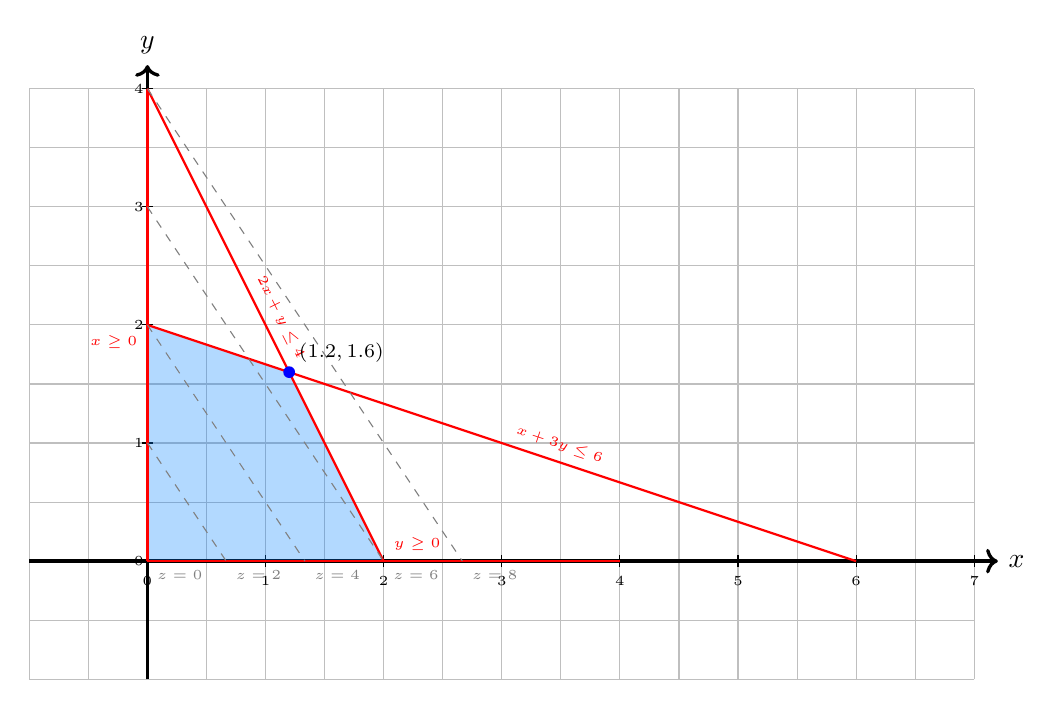
\begin{tikzpicture}[scale = 1.5]
    % Grid and axes
    \draw[gray!50, thin, step=0.5] (-1,-1) grid (7,4);
    \draw[very thick,->] (-1,0) -- (7.2,0) node[right] {$x$};
    \draw[very thick,->] (0,-1) -- (0,4.2) node[above] {$y$};

    % Axis labels
    \foreach \x in {0,...,7} \draw (\x,0.05) -- (\x,-0.05) node[below] {\tiny\x};
    \foreach \y in {0,...,4} \draw (-0.05,\y) -- (0.05,\y) node[left] {\tiny\y};

    % Shaded feasible region
    \fill[blue!50!cyan,opacity=0.3] (0,0) -- (0,2) -- (1.2,1.6) -- (2,0) -- cycle;

    % Constraint lines
    \draw[red,thick] (0,2) -- node[above right,sloped] {\tiny$x + 3y \leq 6$} (6,0);
    \draw[red,thick] (0,4) -- node[above,sloped] {\tiny$2x + y \leq 4$} (2,0);
    \draw[red,thick] (0,0) -- node[below left] {\tiny$x \geq 0$} (0,4);
    \draw[red,thick] (0,0) -- node[above right] {\tiny$y \geq 0$} (4,0);
    
        % Objective function contours
            \draw[dashed,gray] (0,4) -- (8/3,0) node[below right] {\tiny$z=8$};
    \draw[dashed,gray] (0,3) -- (2,0) node[below right] {\tiny$z=6$};
    \draw[dashed,gray] (0,2) -- (4/3,0) node[below right] {\tiny$z=4$};
    \draw[dashed,gray] (0,1) -- (2/3,0) node[below right] {\tiny$z=2$};
    \draw[dashed,gray] (0,0) -- (0,0) node[below right] {\tiny$z=0$};

    % Contour labels
    %\node[gray] at (0.5,3.5) {\tiny$3x + 2y = c$};
    
     \node[blue] at (1.2,1.6) [circle,fill,inner sep=1.5pt]{};

    % Labels for vertices
    \node[black,anchor=south west] at (1.2,1.6) {\scriptsize$(1.2,1.6)$};
\end{tikzpicture}
\end{document}
